\documentclass[a4paper,10pt]{article}
%\documentclass[a4paper,10pt]{scrartcl}

\usepackage[utf8x]{inputenc}

\title{Machine Learning CBC: Assignment Two}
\author{csl209}
\date{}

\usepackage{mathptmx}
\usepackage{graphicx} 

\begin{document}
\LARGE\noindent
\textsc{Machine Learning CBC \\ Assignment Two} \\[1cm]

\large\noindent
Xin Yan Kwek, Darcy Qiu, Charles Koh, and C.S. Rudolf Lai\\ 

\normalsize

\section*{Implementation Details}

We used the one-versus-the rest method to perform multi-class classification. The expected results were remapped such that only labels which matched the target class had a label \texttt{1} while the rest would be mapped to \texttt{0}. This remapped training data is passed to a tree building function, which used the ID3 algorithm to determine the best attribute to branch on by the information gain the attribute offered.

In order to ensure that only each example only has 1 label, we used the result of a 10 cross validation to see which tree had the best precision, the ability to correctly classify its target emotion. In the event where we have a tie, the tree with the highest precision wins it. Should the trees involved in the tie be equally precise, we will randomly select one tree as the winner of the tie.

In the event where all the trees return a negative for an example, we will resolve this ambiguity by selecting the tree which had the lowest precision rate, basing this selection on the greater probability of the tree making a mistake in its classification.

After we had made our function for creating and testing trees, we moved on to validate them with the ten fold validation, confusion matrix, recall rates, precisions rates and lastly the f1 measure.

Ten fold validation was done as described in the manual. This was achieved by finding out the size of a “fold” (One tenth the size of the entire data set). Next the samples were treated as lists. The first “fold” of data would be split from the samples as the test set. The rest would become the training set and used to train 6 trees using the tree making function we made. The testTrees function was used to find the predicted values and compare them with the actual values. Then we update 2 variables, one stores the values for the error estimate, the other, the confusion matrix.

The two variables are populated by first creating 2 empty matrices. The first matrix is a short $2\times1$ matrix for estimate and the confusion matrix is a $6\times6$ matrix. The matrix for error estimates uses the left value to accumulate the error values (no. of wrongly predicted results over total no. of results) and the right value to keep track of how many error estimates have been added (should and will be 10, but I left it there so we could modify easily if needed). The confusion matrix tracks all ten folds and works by incrementing the value with the row no. of the correct value and the column of the predicted value. (i.e. \texttt{confusionMatrix(correctVal,predictedVal)++}).

Once that’s done the test set data that was split off would be concatenated to the back of the list. The cycle (of splitting to concatenation) is then repeated till all the 10 folds are done, resulting in 2 final variables, the confusion matrix which is then used for recall and precision rates and the error estimate result. 

\section*{Pruning}

The \texttt{pruning\_example} function executes three \texttt{MATLAB} tree functions in this sequence: \texttt{treefit}, \texttt{treetest}, and \texttt{treeprune}. First it uses \texttt{treefit} to create a decision tree for predicting responses (targets) as a function of predictors (examples).  The tree is created such that impure nodes will be split as long as there are observations. Using \texttt{treetest}, the expectation of misclassification costs over all terminal nodes is then computed using both the resubstitution method and the 10-fold cross-validation method. Along with the cost, the standard error of each cost value, the terminal node count for each subtree, and an \textit{estimated best level of pruning} is also computed. Using the two estimated best level, we then use \texttt{treeprune} to prune the tree, coming up with two new trees.

\newpage

\section*{Decision Trees}
\begin{figure}[h!]
	\centering
    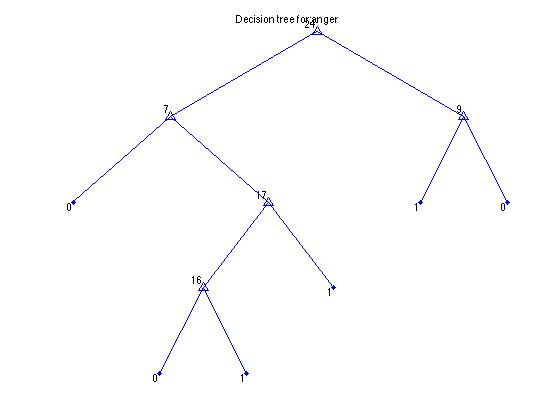
\includegraphics[width=12cm]{anger}
  \caption{The decision tree for \textbf{anger}.}  
\end{figure}

\begin{figure}[h!]
	\centering
    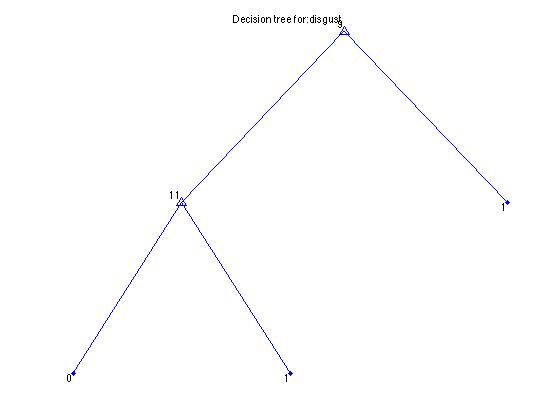
\includegraphics[width=12cm]{disgust}
  \caption{The decision tree for \textbf{disgust}.}  
\end{figure}

\begin{figure}[h!]
	\centering
    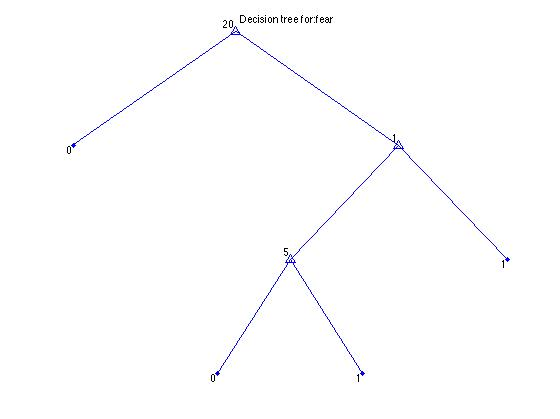
\includegraphics[width=12cm]{fear}
  \caption{The decision tree for \textbf{fear}.}  
\end{figure}

\begin{figure}[h!]
	\centering
    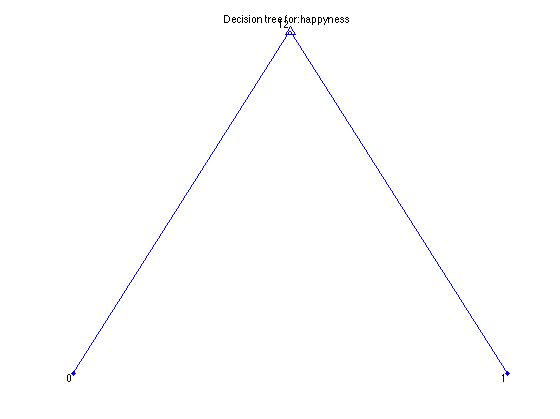
\includegraphics[width=12cm]{happyness}
  \caption{The decision tree for \textbf{happyness}.}  
\end{figure}

\begin{figure}[h!]
	\centering
    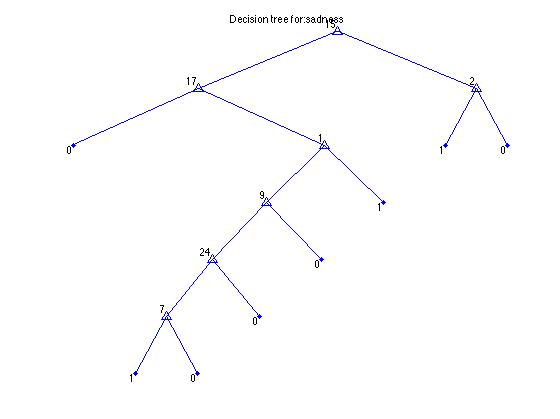
\includegraphics[width=12cm]{sadness}
  \caption{The decision tree for \textbf{sadness}.}  
\end{figure}

\begin{figure}[h!]
	\centering
    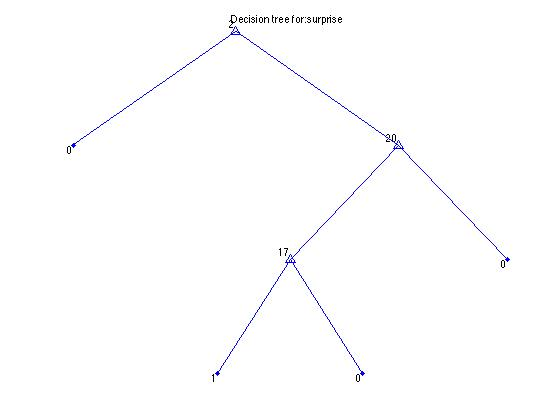
\includegraphics[width=12cm]{surprise}
  \caption{The decision tree for \textbf{surprise}.}  
\end{figure}

\newpage

\section*{Confusion Matrix}
\begin{verbatim}
            anger disgust fear  happiness sadness surprise
  anger     6     0       1     0         1       0
  disgust   0     21      0     0         0       0
  fear      2     0       4     0         1       0
  happiness 0     0       0     23        0       0
  sadness   1     0       0     0         10      1
  surprise  0     0       0     0         0       23
\end{verbatim}

\section*{Recall and Precision Rates}
\begin{verbatim}
              Recall  Precision
  anger       0.7500  0.6667
  disgust     1       1
  fear        0.5714  0.8000
  happiness   1       1
  sadness     0.8333  0.8333
  surprise    1       0.9583
\end{verbatim}

\newpage

\section*{$F_1$ Measure}
\begin{verbatim}
  anger     0.7059
  disgust   1
  fear      0.6667
  happiness 1
  sadness   0.8333
  surprise  0.9787
\end{verbatim}

\end{document}
